\documentclass[11pt,a4paper]{article}
\usepackage[utf8]{inputenc}
\usepackage[T1]{fontenc}
\usepackage[spanish,es-tabla,es-noshorthands]{babel}
\usepackage{lmodern}
\usepackage[margin=2.25cm]{geometry}
\usepackage{booktabs,longtable,amsmath,microtype,graphicx,pdflscape}
\usepackage{hyperref}
\hypersetup{colorlinks=true,linkcolor=black,urlcolor=blue,pdftitle={Optimización medida de MPI en 96 núcleos}}
\setlength{\parskip}{5pt}
\setlength{\parindent}{0pt}
\begin{document}
\begin{titlepage}
\centering
{\Large Universidad Nacional de San Agustín\par}
\vspace{0.4cm}
{\large Ciencia de la Computación\par}
\vspace{2cm}
\rule{\linewidth}{0.5mm}\par
\vspace{0.4cm}
{\Huge\bfseries Optimización medida de MPI\par}
\vspace{0.3cm}
{\Large Difusión, topología y multiplicación de matrices\par}
\vspace{0.4cm}
\rule{\linewidth}{0.5mm}\par
\vspace{2cm}
{\large Extensión reproducible del proyecto\par}
\vspace{0.3cm}
\url{https://github.com/dtamotu/cluster-mpi-96-optimizaciones}\par
\vspace{2cm}
\begin{minipage}[t]{0.52\linewidth}\raggedright
\textbf{Integrantes:}\\
Paredes Malaga José Carlos\\
Jheeremy Manuel Alvarez Astete\\
Jose Alejandro Machaca Muñiz\\
David Tamo Turpo\\
Wilson Ramos
\end{minipage}\hfill
\begin{minipage}[t]{0.4\linewidth}\raggedleft
\textbf{Curso:}\\
Computación Paralela y Distribuida\\[0.2cm]
\textbf{Profesor:}\\
Alvaro Henry Mamani Aliaga
\end{minipage}
\vfill
{\large Arequipa, Perú --- septiembre de 2026\par}
\end{titlepage}

\tableofcontents
\clearpage
\section{Pregunta y punto de partida}
Se investiga si pueden reducirse más los tiempos medidos al multiplicar matrices en un clúster de cuatro computadoras, cada una con 24 núcleos. La batería anterior, preservada en \path{datos/ampliada/resultados_consolidados.csv}, registró para $N=3072$ tiempos de 0.547 s con 24 procesos locales, 6.148 s con 96 procesos por Ethernet y 99.945 s con 96 procesos por Wi-Fi. Con 96 procesos, el cálculo local máximo fue 0.104 s por Ethernet y 0.139 s por Wi-Fi; el costo dominante se registró en distribución y espera. Son corridas individuales, no distribuciones estadísticas.

La corrida histórica de 906.351 s con ocho procesos registró 889.744 s en \texttt{MPI\_Bcast}. No es una repetición de la batería de 96 procesos: también cambiaron ejecutable, algoritmo local, asignación y condiciones de red. La ausencia de la opción explícita \texttt{vader} no demuestra que Open MPI enviara tráfico local por TCP; Open MPI 4.x puede escoger memoria compartida por defecto\footnote{\url{https://www.open-mpi.org/faq/?category=tcp}}.

\section{Diseño de experimentos}
Cada corrida usa la misma matriz determinista, el núcleo local \texttt{tiled} y una sola ejecución MPI a la vez. El script de esta carpeta guarda comando, salida, fecha, versión de Open MPI y contadores TX/RX de cada nodo. Los resultados se identifican por red, procesos, nodos, variante y repetición. El orden cambia de forma determinista entre repeticiones. Las cinco repeticiones permiten describir dispersión, pero no garantizan condiciones de red idénticas.

\begin{enumerate}
\item \textbf{Uno frente a cuatro nodos.} Se comparan 24 procesos locales y 96 procesos en cuatro nodos, tanto por Ethernet como por Wi-Fi.
\item \textbf{Difusión jerárquica explícita.} En \texttt{1d-hier}, los líderes de nodo difunden $B$ entre sí y cada líder vuelve a difundirla localmente. \texttt{1d} usa una colectiva global. Se miden por separado \texttt{Scatterv} y \texttt{Bcast}. El cálculo y los datos son los mismos.
\item \textbf{Difusión aislada.} Se transmite una matriz de 75.497 MB con 16 procesos: todos en un nodo o cuatro en cada uno de cuatro nodos. Se contrastan la colectiva global, la jerárquica y dos algoritmos solicitados al componente \texttt{tuned}: \texttt{knomial} y \texttt{scatter\_allgather}. Las opciones disponibles se verificaron en Open MPI 4.1.6 mediante \texttt{ompi\_info}.
\item \textbf{Distribución 2D.} Se compara el 1D con SUMMA 2D a $P=64$ y $N=3072$. El programa 2D actual exige $P=q^2$ y $N$ divisible por $q$, de modo que 96 procesos no son una comparación válida sin modificar la partición.
\item \textbf{Tamaño mayor.} Por Ethernet se miden matrices de $N=6144$ y $N=7168$ con 24 y 96 procesos. Esto busca un posible cruce entre uno y cuatro nodos dentro de tamaños compatibles con la memoria por proceso. No se extrapola hasta tamaños que la implementación 1D no puede alojar.
\item \textbf{Trapecio asimétrico.} Se corrige la contribución del extremo $f(1)/2$ que faltaba en el programa experimental. Se comparan partición simétrica y ponderada para $n=10^8$ y $10^{11}$, con 24 y 96 procesos, por Ethernet. La ponderación fija asigna peso 1.2658 a los primeros ocho rangos de cada nodo y 1 a los demás; es una hipótesis previa, no una calibración nueva. Los logs guardan error absoluto de la integral, afinidad de rangos y tiempos máximos y mínimos de cálculo.
\end{enumerate}

La cifra de tráfico es la suma de bytes TX de las interfaces de los nodos participantes durante cada ventana, en MB decimales. También se guardan RX y los valores antes/después. Estas cifras pueden incluir SSH, control MPI y tráfico ajeno. No representan por sí solas bytes útiles de una colectiva ni uso total del aire Wi-Fi. Los máximos de fases pueden corresponder a procesos distintos y no se suman para reconstruir el tiempo total.

Para $N=3072$, una matriz de dobles ocupa $8N^2=75.497472$ MB. Si una difusión transmitiera una copia de $B$ hacia cada uno de los tres nodos remotos, la carga útil ideal entre nodos sería $3\times75.497472=226.492416$ MB. Esta es una referencia de volumen útil, no un contador medido ni una identificación del algoritmo interno de Open MPI.

\section{Resultados}
Se guardaron 118 intentos, de los cuales 118 terminaron y entregaron una línea de resultado válida.

\begin{landscape}\footnotesize\renewcommand{\arraystretch}{1.0}
\input{tablas_optimizacion}
\end{landscape}

\begin{figure}[htbp]\centering
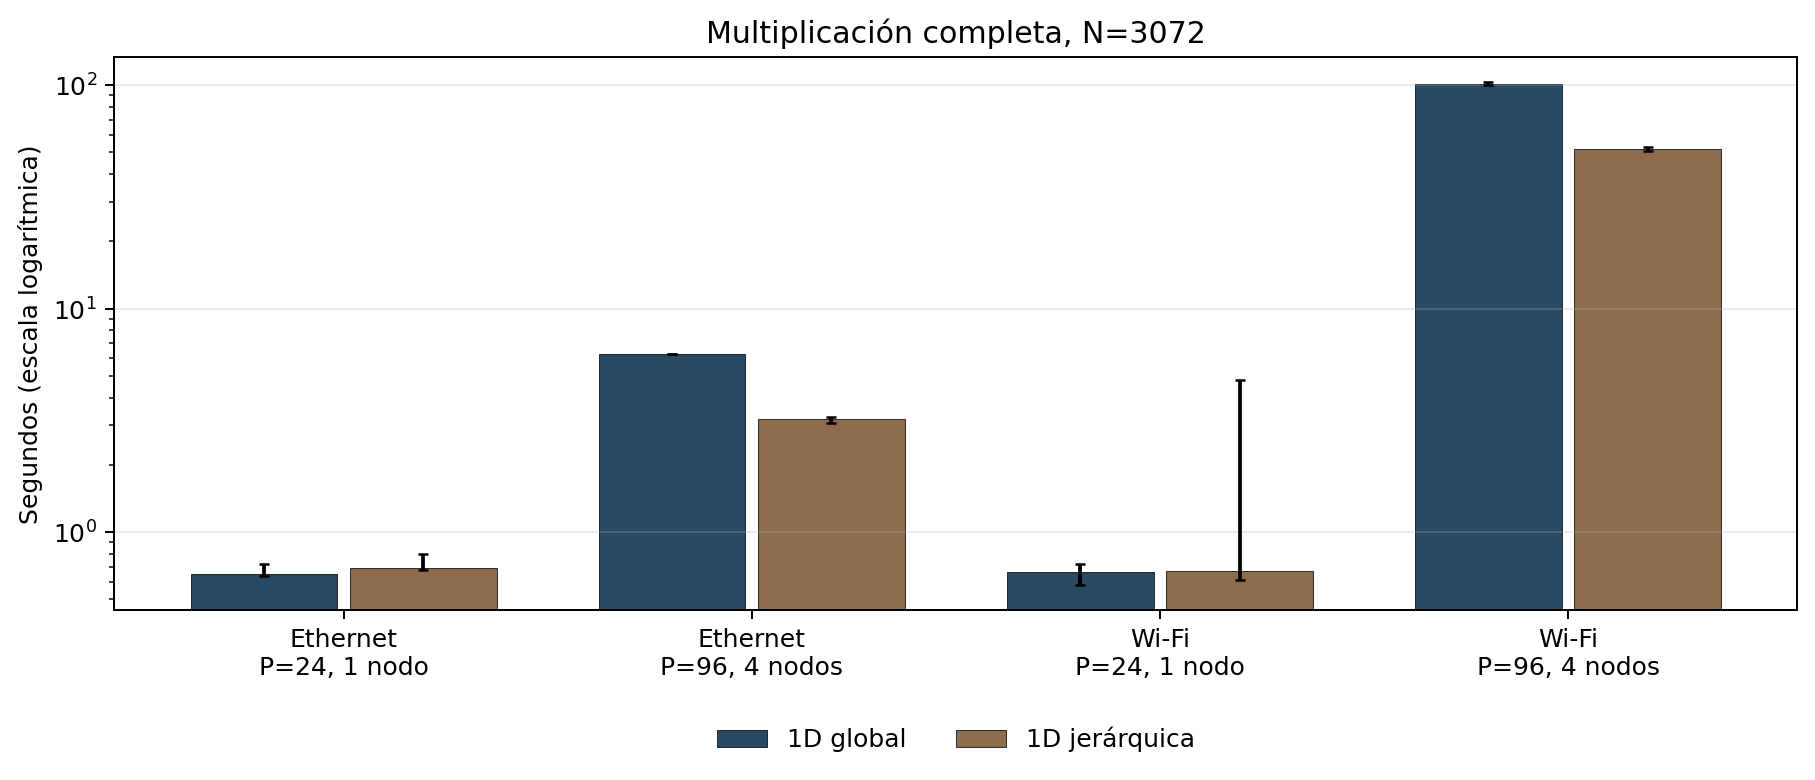
\includegraphics[width=\linewidth]{img/optimizacion_matrices.png}
\caption{Tiempo del programa completo, mediana y rango de las corridas válidas. La escala vertical es logarítmica.}
\end{figure}
\begin{figure}[htbp]\centering
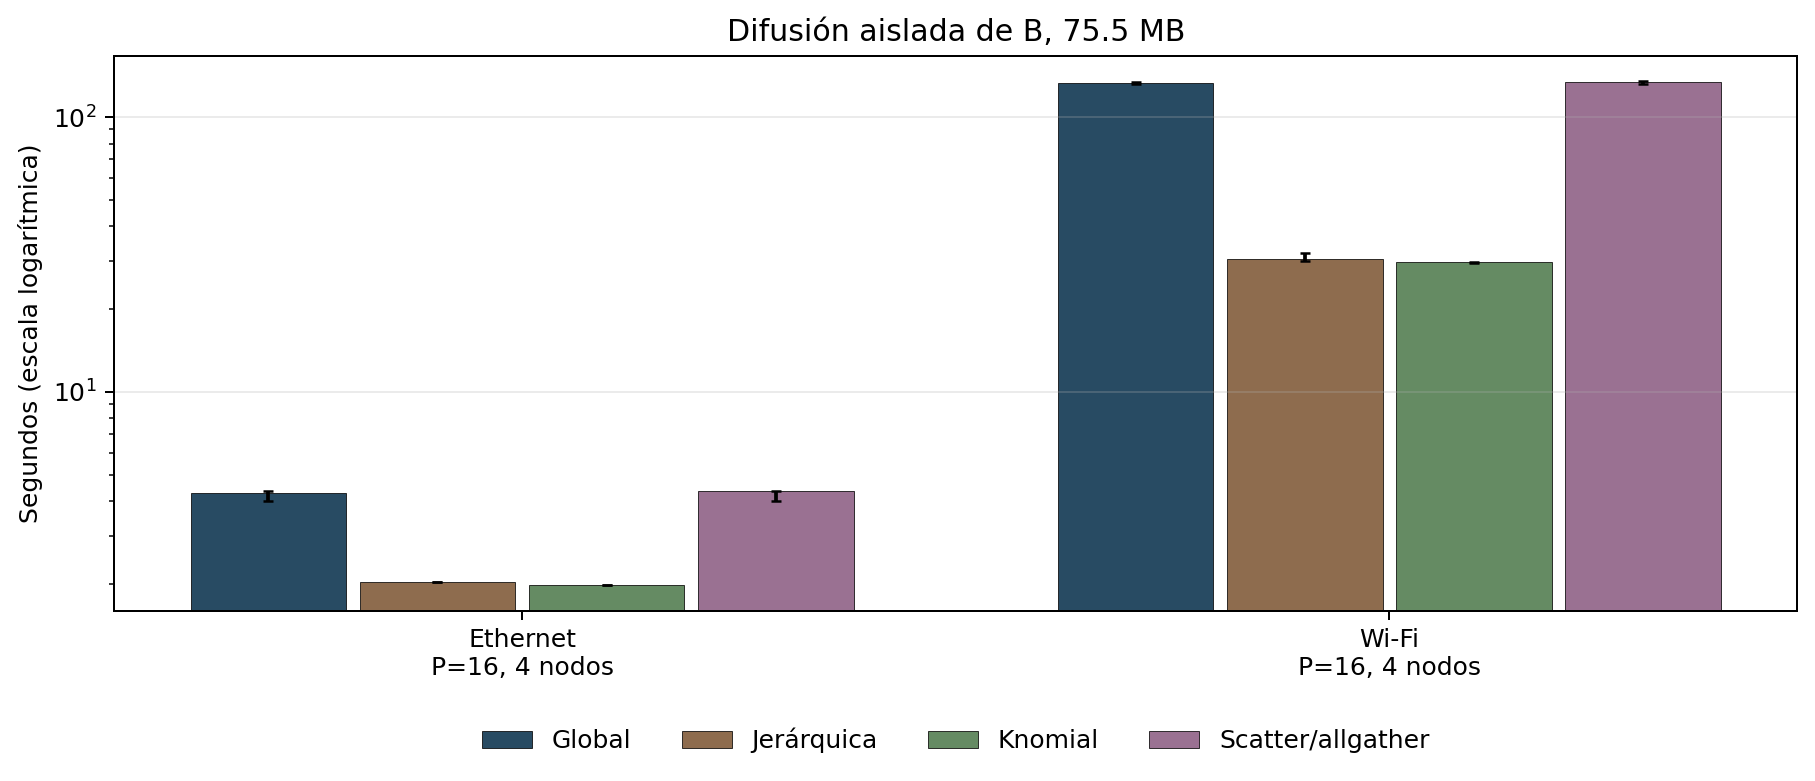
\includegraphics[width=\linewidth]{img/optimizacion_bcast.png}
\caption{Difusión aislada entre cuatro nodos. La escala vertical es logarítmica; las barras de error muestran mínimo y máximo.}
\end{figure}
\begin{figure}[htbp]\centering
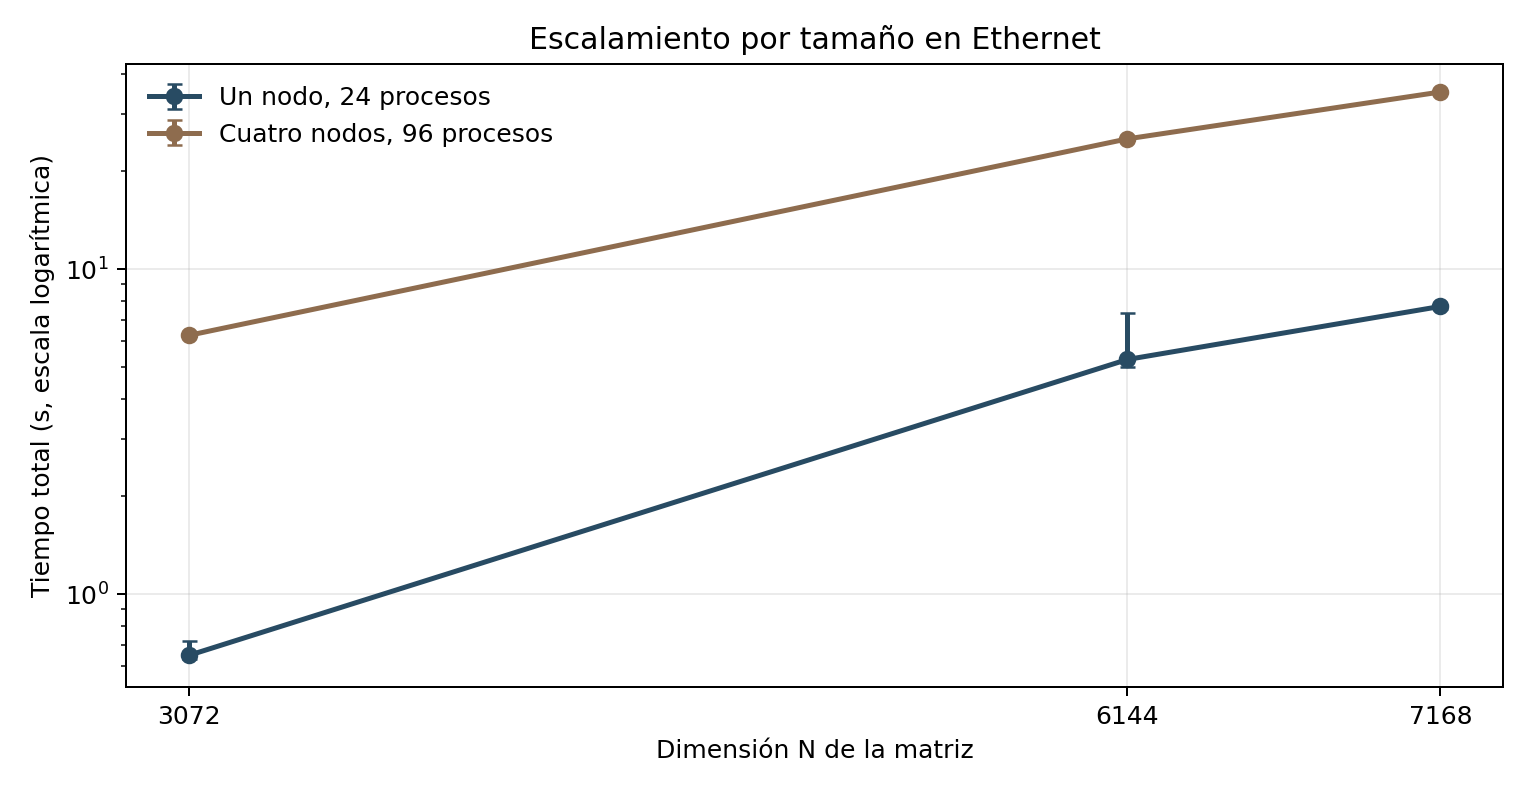
\includegraphics[width=0.88\linewidth]{img/optimizacion_tamano.png}
\caption{Tiempo de matrices 1D por Ethernet, con uno o cuatro nodos. Los puntos muestran medianas y los extremos de las barras el rango observado.}
\end{figure}

La columna $T$ corresponde a \texttt{T\_Total} del programa completo o a \texttt{T\_Bcast} del microbenchmark. Por tanto, se comparan tiempos solo dentro de cada tipo de prueba. Los logs de matrices conservan además la suma diagonal y una suma ponderada de la matriz final; el microbenchmark comprueba que las huellas de 64 bits de los búferes coinciden entre procesos.

\section{Comparaciones principales}
En Ethernet, la difusión jerárquica explícita frente a 1D por defecto a $P=96$ dio un cociente de tiempos 1.95\,veces y un cociente de TX agregados 2.11\,veces. Un valor mayor que 1 favorece la variante jerárquica. El máximo de la fase Bcast pasó de 5.611 a 2.474 s.


En Wi-Fi, la difusión jerárquica explícita frente a 1D por defecto a $P=96$ dio un cociente de tiempos 1.96\,veces y un cociente de TX agregados 2.13\,veces. Un valor mayor que 1 favorece la variante jerárquica. El máximo de la fase Bcast pasó de 88.904 a 40.272 s.


En Ethernet, 1D frente a SUMMA 2D, ambos con $P=64$, dio un cociente de tiempos 0.57\,veces y un cociente de TX agregados 0.53\,veces. Un valor menor que 1 favorece 1D.


En Wi-Fi, 1D frente a SUMMA 2D, ambos con $P=64$, dio un cociente de tiempos 0.59\,veces y un cociente de TX agregados 0.51\,veces. Un valor menor que 1 favorece 1D.


En la difusión aislada por Ethernet, la colectiva global frente a la jerárquica dio un cociente de tiempo 2.11\,veces y de TX agregado 4.33\,veces.


En la difusión aislada por Wi-Fi, la colectiva global frente a la jerárquica dio un cociente de tiempo 4.37\,veces y de TX agregado 4.41\,veces.


Con 16 procesos y difusión global por Ethernet, cuatro nodos frente a uno dieron un cociente 37.08\,veces.


En Ethernet, cuatro nodos con 96 procesos frente a un nodo con 24 procesos dieron un cociente $T_{96}/T_{24}$ de 9.65\,veces. Aquí un valor mayor que 1 favorece un nodo.


En Wi-Fi, cuatro nodos con 96 procesos frente a un nodo con 24 procesos dieron un cociente $T_{96}/T_{24}$ de 151.70\,veces. Aquí un valor mayor que 1 favorece un nodo.


Para $N=6144$ por Ethernet, $T_{96}/T_{24}$ fue 4.77\,veces.


Para $N=7168$ por Ethernet, $T_{96}/T_{24}$ fue 4.57\,veces.


Trapecio con $n=10^8$ y $P=24$: $T_{sim}/T_{asim}$ fue 1.70\,veces.


Trapecio con $n=10^8$ y $P=96$: $T_{sim}/T_{asim}$ fue 1.07\,veces.


Trapecio con $n=10^{11}$ y $P=24$: $T_{sim}/T_{asim}$ fue 1.05\,veces.


Trapecio con $n=10^{11}$ y $P=96$: $T_{sim}/T_{asim}$ fue 0.97\,veces.



\section{Interpretación y límites}
Una mejora de \texttt{1d-hier} frente a \texttt{1d} sería evidencia favorable a agrupar la difusión por nodo \emph{en esta topología y versión}, pero no demuestra qué algoritmo usó la colectiva global internamente. La variante jerárquica todavía reserva una copia completa de $B$ por proceso. Reducir esa memoria exigiría otra implementación, por ejemplo una ventana compartida por nodo.

La comparación 2D usa el mismo número de procesos que 1D en sus dos ramas, y controla la corrección con dos sumas de verificación. SUMMA realiza varios pasos de difusión de paneles y añade empaquetamiento; por eso se informa su tiempo completo además del tráfico. No debe extrapolarse directamente de 64 a 96 procesos. La optimización del núcleo aritmético, por ejemplo con una biblioteca BLAS, sería una pregunta separada; en la batería original de 96 procesos el cálculo ocupó una fracción muy pequeña del tiempo total.

En el trapecio, la ponderación supone que ciertos rangos corresponden a núcleos P y otros a núcleos E. Su utilidad debe interpretarse junto con la afinidad real registrada para cada corrida; una mejora de tiempo por sí sola no demuestra que la clasificación de núcleos fuera correcta.

Para $n=10^8$, el tiempo interno de trapecio es de milisegundos. Su variación relativa puede ser grande, por lo que $n=10^{11}$ es la comparación más informativa para el reparto de carga.

\section{Reproducción}
Desde esta carpeta:
\begin{itemize}
\item \path{./preparar.sh} compila los programas y copia los ejecutables al directorio temporal de cada nodo.
\item \path{experimentos.py} ofrece \texttt{plan}, \texttt{smoke}, \texttt{run} y \texttt{extra}; los dos últimos guardan las baterías nuevas.
\item \path{auditar_resultados.py} contrasta CSV y logs, y genera \texttt{SHA256SUMS}.
\item \path{generar_informe_optimizacion.py} reconstruye este informe y su PDF desde los CSV, sin ejecutar MPI.
\item \path{./ejecutar_todo.sh} reúne esos pasos.
\end{itemize}

El código, los scripts, las fuentes del informe, los CSV y los logs están en esta carpeta local. En los otros nodos solo se alojan temporalmente los ejecutables necesarios para \texttt{mpirun}.
\end{document}
